\documentclass[12pt, twoside]{article}
\usepackage{jmlda}
\newcommand{\hdir}{.}



\begin{document}

\title
    [Обоснованность применения DTW к пространственно-временным объектам] % краткое название; не нужно, если полное название влезает в~колонтитул
    {Теоретическая обоснованность применения метрических методов классификации с использованием динамического выравнивания (DTW) к пространственно-временным объектам}
\author
    [И.\,О.~Автор] % список авторов (не более трех) для колонтитула; не нужен, если основной список влезает в колонтитул
    {А.\,А.~Харь, Г.~Моргачев, А.~Гончаров} % основной список авторов, выводимый в оглавление
    [А.\,А.~Харь, Г.~Моргачев, Г.~Гончаров] % список авторов, выводимый в заголовок; не нужен, если он не отличается от основного
\email
    
\thanks
    {Работа выполнена при
     %частичной
     финансовой поддержке РФФИ, проекты \No\ \No 00-00-00000 и 00-00-00001.}
\organization
    
\abstract
    {Решается задача выравнивания пространственно-временных рядов, строится функция расстояния. Для этого используется метод динамического выравнивания. В работе исследуется корректность метода динамического выравнивания и его модификаций к пространственно-временным рядам. При доказательстве, проверяют, что функция, создаваемая алгоритмом динамического выравнивания, является ядром. Проверка этого факта осуществляется при помощи теоремы Мерсера, основная часть которой заключается в проверке матрицы попарных расстояний на неотрицательную определенность. Также производится анализ зависимости качества классификации методом опорных векторов и методом k-ближайших соседей от различных функций.
	
\bigskip
\noindent
\textbf{Ключевые слова}: \emph {динамическое выравнивание; пространственно-временные ряды; ядро функции; теорема Мерсера; функция расстояния; функция расстояния; метод опорных векторов; метод k-ближайших соседей}
}


%данные поля заполняются редакцией журнала
\doi{10.21469/22233792}
\receivedRus{01.01.2017}
\receivedEng{January 01, 2017}

\maketitle
\linenumbers

\section{Введение}
{Функция расстояния между временными рядами может быть задана различными
способами: Евклидово расстояние \cite{Evklid}, метод динамического выравнивания временных
рядов \cite{DTW1, DTW2}, метод, основанный на нахождение наибольшей общей последовательности \cite{MaxSequence}.
В \cite{Noise} показано, что разность между значениями временного ряда, соответствующими различным временным отсчетам, не может рассматриваться в качестве описания расстояния между двумя объектами: эта метрика чувствительна к
шуму и локальным временным сдвигам. Предлагается использовать метод динамического выравнивания временных рядов (англ. Dynamic Time
Warping) \cite{DTW}. Как показано в \cite{Thebestmethod}, этот метод находит наилучшее соответствие между
двумя временными рядами, если они нелинейно деформированы друг относительно
друга -- растянуты, сжаты или смещены вдоль оси времени. Метод DTW используется для определения сходства между ними и введения расстояния между двумя временными рядами.\\

На данный момент существуют теоретические обоснования (создаваемая алгоритмом функция точно аппроксимирует аналитическую функцию) применения DTW лишь для некоторых временных объектов, например, для дизартрического распознавания речи с разреженными обучающими данными \cite{DisartreSpeech}. В этой статье теоретически обосновывается его применение для пространственно-временных объектов. Исследование проводится на данных \cite{Data}.\\


Алгоритм построения оптимальной разделяющей гиперплоскости -- алгоритм линейной классификации \cite{SVM_Bennett}. В основе создания же нелинейного классификатора лежит замена скалярного произведения $\langle x, x' \rangle$ на функцию ядра $K(x, x')$. Таким образом осуществляется переход в спрямляющее пространство (kernel trick), который позволяет построить нелинейные разделители. Если изначально выборка была линейно неразделимой, то при удачном выборе ядра можно избавить от этой проблемы. Это позволяет применять линейные алгоритмы классификации (SVM) в случаях, когда выборка не разделяется линейно. Критерием функции ядра является теорема Мерсера \cite{Mercer},\\




}





\section{Постановка задачи}
В работе мы будем проверять выполнение условий теоремы Мерсера на разных данных для разных модификаций DTW. То есть, следующие два условия для функции $K(x,x')$, порожденной DTW:\\
$\bullet \ K(x,x') = K(x',x)$\\
$\bullet \ \int\limits_X \int\limits_X K(x,x')g(x)g(x')dxdx' \geq 0 \ \ \ \forall g:X \rightarrow \mathbb{R}$\\
Последнее условие эквивалентно тому, что для любых наборов $\{ x_1, \ldots, x_n \}$ матрица $K = ||K(x_i,x_j)||_{i,j}$ неотрицательно определена: $v^TKv \geq 0 \ \ \forall v \in \mathbb{R}^n$\\

В нашей задаче мы будем исследовать, насколько качественно функции (являющиеся ядрами или нет), полученные в результате DTW, подставленные в алгоритм SVM (Support Vector Machine), классифицируют объекты. Для начала рассмотрим задачу классификации объектов $X \in \mathbb{R}^n$ на два непересекающихся класса $Y = \{-1, +1 \}$. Обучающая выборка $X^l = (x^j,y^j)_{j=1}^l$ Линейный классификатор будет иметь вид:\\
$a(x) = sign(\sum\limits_{i=1}^n w_ix_i - w_0) = sign(\langle w,x \rangle - w_0)$\\
Тут использованы обозначения: $x = (x_1, \ldots, x_n) $ --  признаковое описание объекта $x$, $w = ( w_1, \ldots , w_n)  \in \mathbb{R}^n $ и $w_0 \in \mathbb{R}$ являются, так называемыми весами, являющимися параметрами алгоритма.\\
Заметим, что $\langle w,x \rangle = w_0$ задает в пространстве гиперплоскость, которая разделяет классы.

Заметим, что линейный классификатор $a(x)$ не изменится если $w$ и $w_0$ умножить на одну и ту же положительную константу. Поэтому произведем нормировку наиболее удобным для нас способом: чтобы для всех ближайших к раздеяющих гиперплоскости объектов $x^j \in X^l \hookrightarrow \langle w, x^j \rangle - w_0 = y^j$ . Таким образом получим для всех $x^j \in X^l$:\\
$\langle w, x^j \rangle - w_0 \ \begin{cases}  \leq -1, \ if \ y^j = -1 \\ \geq 1, \  if \  y^j = +1 \end{cases}$\\
$-1 < \langle w,x \rangle - w_0 < 1$ задает полосу, которая разделяет классы.  Внутри этой полосы нет ни одной точки обучающей выборки $X^l$, на ее границе лежат точки, ближайшие к разделяющей гиперплоскости. Сама гиперплоскость проходит ровно посередине полосы.
Мы хотим добиться максимальной ширины $h$ этой полосы (для более качественной классификации). Пусть точки $x_{-}, x^{+}$ -- соответственно точки классов $-1, +1$, лежащие на границе полосы, тогда:
$h = \dfrac{1}{||w||} \langle x_{+} - x_{-}, w \rangle = \dfrac{\langle x_{+}, w \rangle - \langle x_{-}, w \rangle}{||w||} = \dfrac{(w_0 + 1) - (w_0 - 1)}{||w||} = \dfrac{2}{||w||}$\\

Таким образом, нам необходимо решить следующую задачу оптимизации:\\
$\begin{cases}\frac{1}{2} \langle w, w \rangle \rightarrow min \\ (\langle w, x^j \rangle - w_0)y^j \geq 1 \ \ i = 1, \ldots, l \end{cases}$\\
Решаем данную задачу при помощи теоремы Каруши-Куна Таккера:\\
$\begin{cases} L(w,w_0,\lambda) = \frac{1}{2}\langle w, w \rangle - \sum\limits_{j=1}^l \lambda_j\big((\langle w, x^j \rangle - w_0)y^j -1\big) \rightarrow \min_{w,w_0}\max_{\lambda} \\ \lambda \geq 0 \\ \lambda_j(\langle w, x^j \rangle - w_0) = 0 \ \ j = 1, \ldots, l \end{cases}$\\
$\lambda = (\lambda_1, \ldots, \lambda_l)$ -- вектор двойственных переменных\\
Необходимым условием седловой точки Лагранжиана $L$, является равенство нулю его градиента, отсюда получаем:
 $w  = \sum\limits_{j=1}^l\lambda_jy^jx^j, \ \sum\limits_{j=1}^l \lambda_jy^j = 0 \ \ \ \ \ (1)$\\
Из первого следует, что вектор весов $w$ является линейной комбинацией таких векторов обучающей выборки $X^l$, для которых соответствующее $\lambda_j \neq 0$. Согласно условию дополнящей нежесткости, так как $\lambda_j \neq 0$, исходные ограничения типа неравенств должны превратиться в равенства, значит, эти объекты (векторы) находятся на границе полосы. Вектора для которых $\lambda_j = 0$ не лежат на границе, и не участвуют в сумме, значит, фалгоритм не изменился бы, если их не было бы в выборке.\\

Объект $(x_j, y_j) \in X^l$, для которого $\lambda_j > 0$ и $\langle w, x^j \rangle - w_0 = y^j$ назовем опорным вектором (англ. support vector)\\

Подставим $(1)$ обратно в выражение для Лагранжиана, получим:\\
$\begin{cases}
-L = -\sum\limits_{j=1}^l\lambda_j + \frac{1}{2}\sum\limits_{i=1}^l\sum\limits_{j=1}^l \lambda_i\lambda_jy^iy^j\langle x^i, x^j \rangle \rightarrow \min_{\lambda} \\
\lambda \geq 0 \ \ \ \ \ \ \ \ \ \ \ \ \ \ \ \ \ \  \ \ \ \ \ \ \ \ \ \ \ \ \ \ \ \ \ \ \ \ \ \ \ \ \ \ \ \ \ \ \ \ \ \ \ \ \ \ \ \ \ \  \ \ \ \ \ \ \ \ \ (2)\\
\sum\limits_{j=1}^ \lambda_j y^j = 0
\end{cases}$\\
Полученная задача имеет единственное решение, поскольку целевая функция является квадратичным функционалом, имеющим неотрицательно определенную квадратичную форму, значит, является выпуклым, ограничения также выпуклы.\\

После решения задачи мы можем определить вектор $w$ по формуле $w  = \sum\limits_{j=1}^l\lambda_jy^jx^j$ и $w_0 = med\{\langle w, x^j \rangle  - y^j: \ \lambda_j > 0, \ j = 1, \ldots, l\}$\\

Тогда получим: $a(x) = sign \big(\sum\limits_{j=1}^l\lambda_jy^j\langle x^j,x \rangle - w_0 \big)$\\

Вопрос о решении двойственной задачи $(2)$ все еще остается открытым.

Все эти рассуждения имеют место в случае, когда выборка линейно разделима, если же она не является таковой, то необходимо перейти в пространство большей размерности, где уже она будет линейно разделима. Этот переход будет осуществляться засчет функции ядра. Скалярные произведения $\langle x,x' \rangle$, таким образом, везде заменятся на значение функции ядра в соответствующих двух точках $K(x,x')$.


\section{Экcперимент}\\
Производится тестирование различных модификаций алгоритма DTW на различных данных \cite{Data}, затем осуществляется проверка того, является ли полученная в результате работы алгоритма функция ядром (при помощи Теоремы Мерсера). 

Строятся выравнивающие пути попарно между пятью временными рядами:

\begin{figure}[H]
\centering
\begin{minipage}{0.66\textwidth}
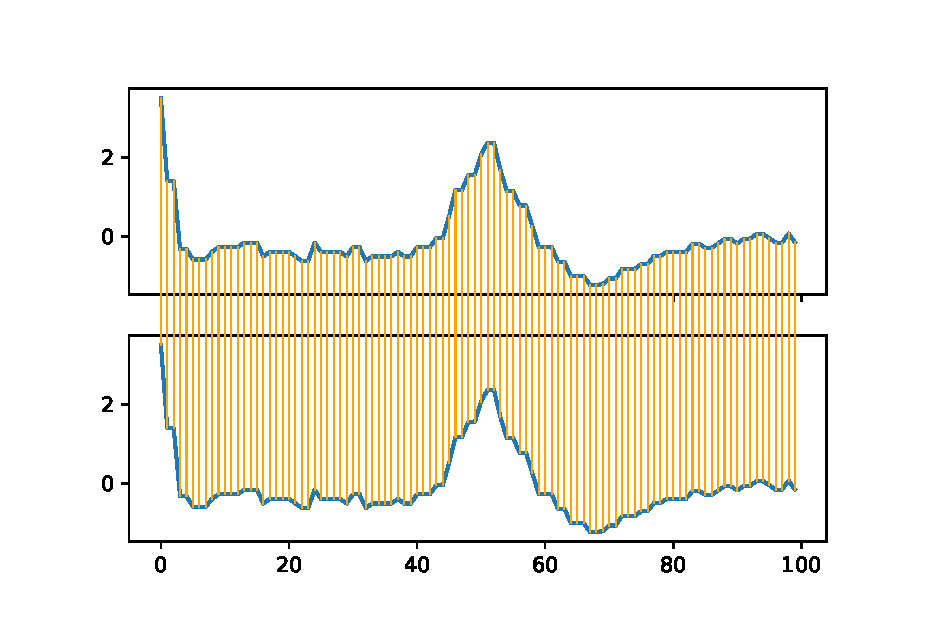
\includegraphics[width = \textwidth]{warp[0][0].eps}
\end{minipage}%
\caption{ . 1 и 1 временные ряды}
\label{fig:2}
\end{figure}

\begin{figure}[H]
\centering
\begin{minipage}{0.66\textwidth}
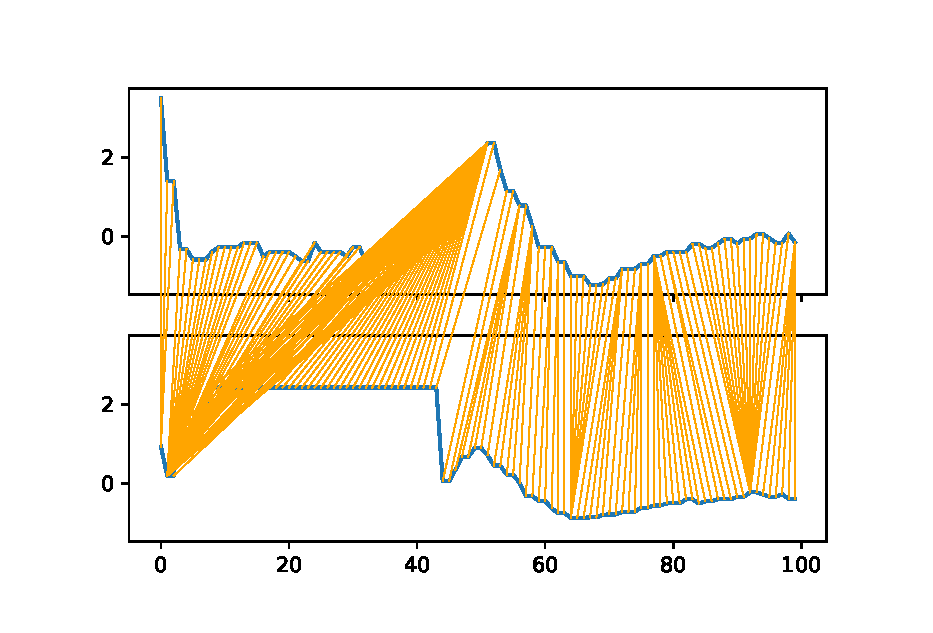
\includegraphics[width = \textwidth]{warp[0][1].eps}
\end{minipage}%
\caption{ . 1 и 2 временные ряды}
\label{fig:2}
\end{figure}

\begin{figure}[H]
\centering
\begin{minipage}{0.66\textwidth}
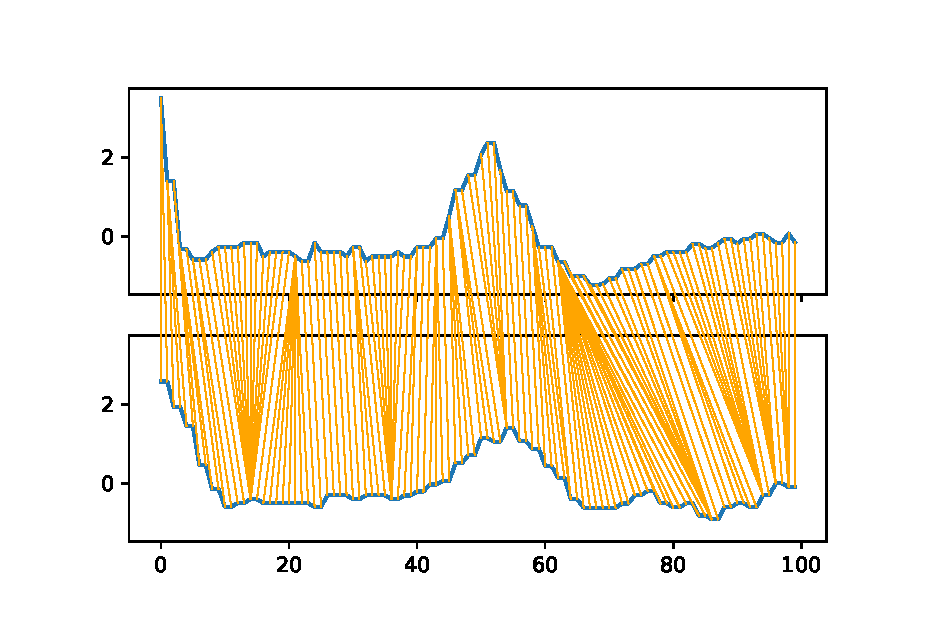
\includegraphics[width = \textwidth]{warp[0][2].eps}
\end{minipage}%
\caption{ . 1 и 3 временные ряды}
\label{fig:2}
\end{figure}

\begin{figure}[H]
\centering
\begin{minipage}{0.66\textwidth}
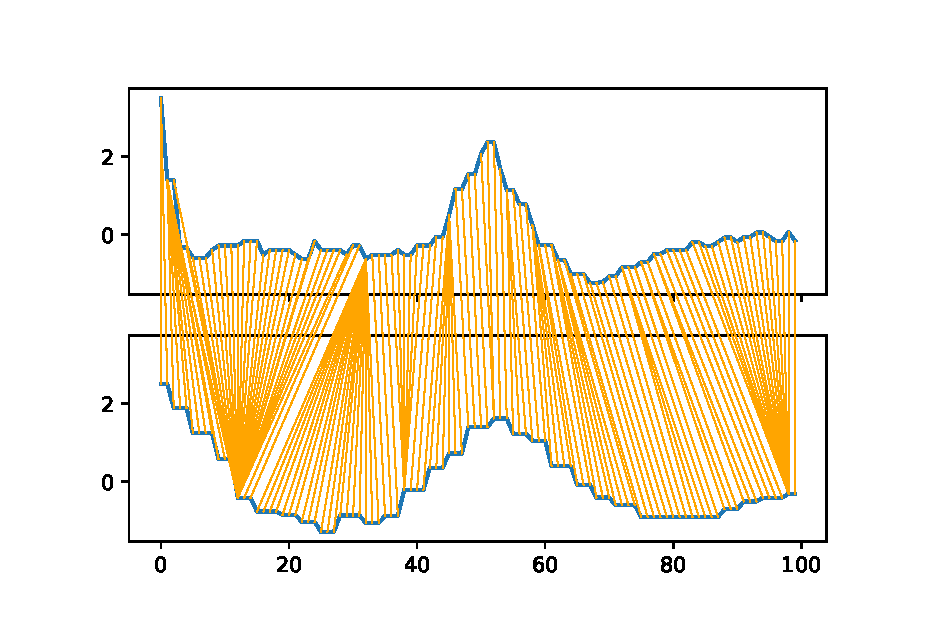
\includegraphics[width = \textwidth]{warp[0][3].eps}
\end{minipage}%
\caption{ . 1 и 4 временные ряды}
\label{fig:2}
\end{figure}

\begin{figure}[H]
\centering
\begin{minipage}{0.66\textwidth}
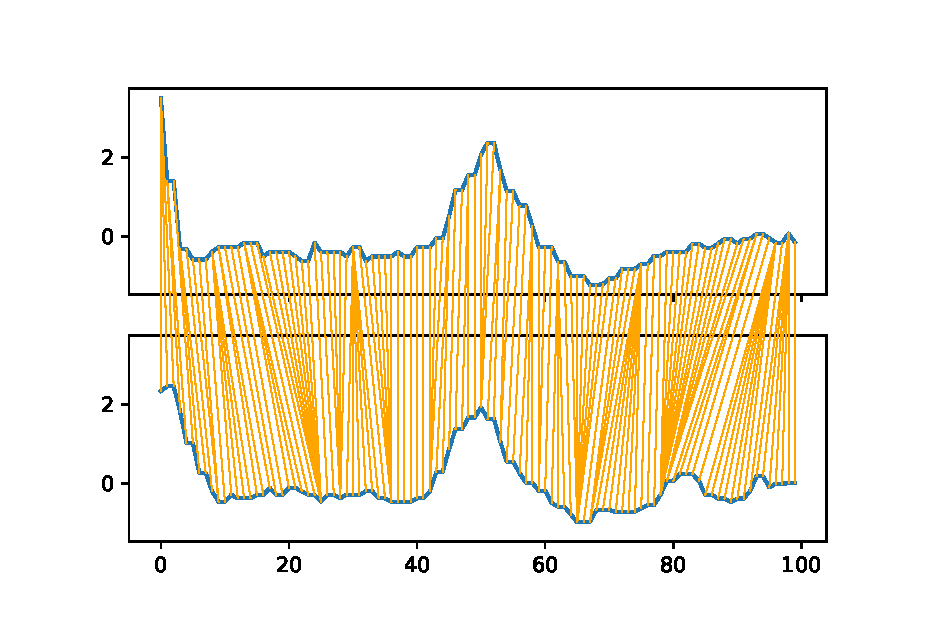
\includegraphics[width = \textwidth]{warp[0][4].eps}
\end{minipage}%
\caption{ . 1 и 5 временные ряды}
\label{fig:2}
\end{figure}

\begin{figure}[H]
\centering
\begin{minipage}{0.66\textwidth}
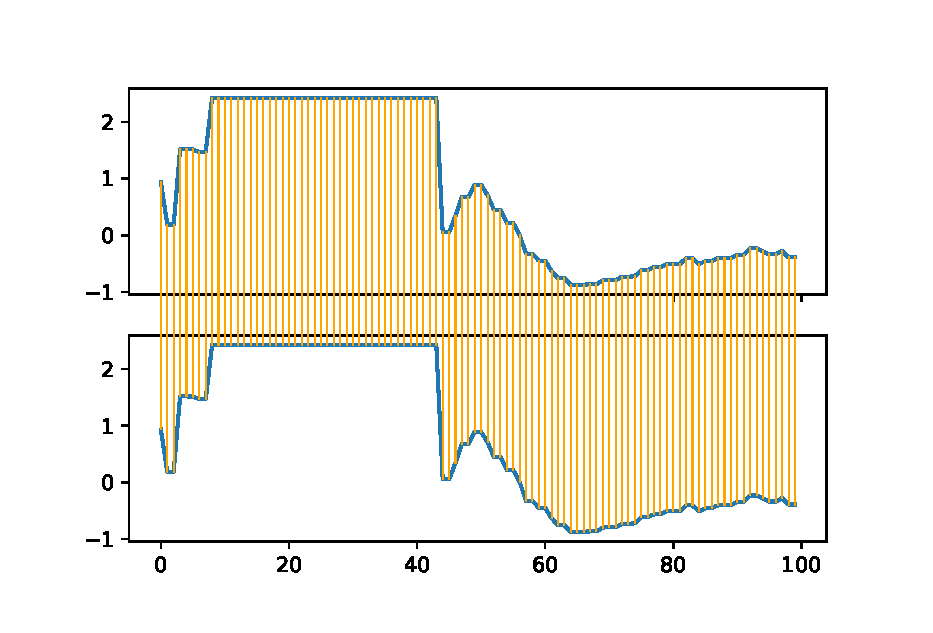
\includegraphics[width = \textwidth]{warp[1][1].eps}
\end{minipage}%
\caption{ . 2 и 2 временные ряды}
\label{fig:2}
\end{figure}

\begin{figure}[H]
\centering
\begin{minipage}{0.66\textwidth}
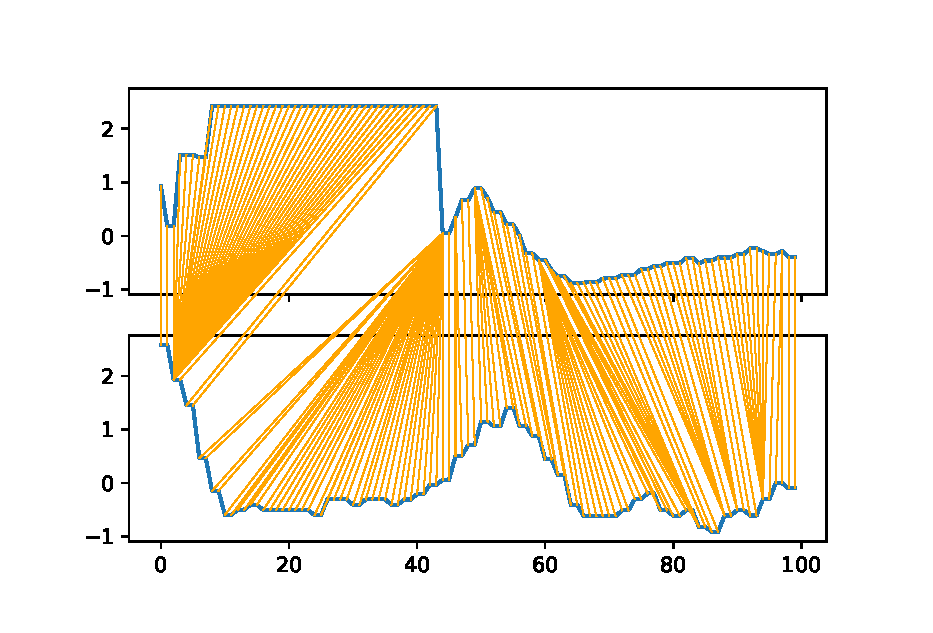
\includegraphics[width = \textwidth]{warp[1][2].eps}
\end{minipage}%
\caption{ . 2 и 3 временные ряды}
\label{fig:2}
\end{figure}

\begin{figure}[H]
\centering
\begin{minipage}{0.66\textwidth}
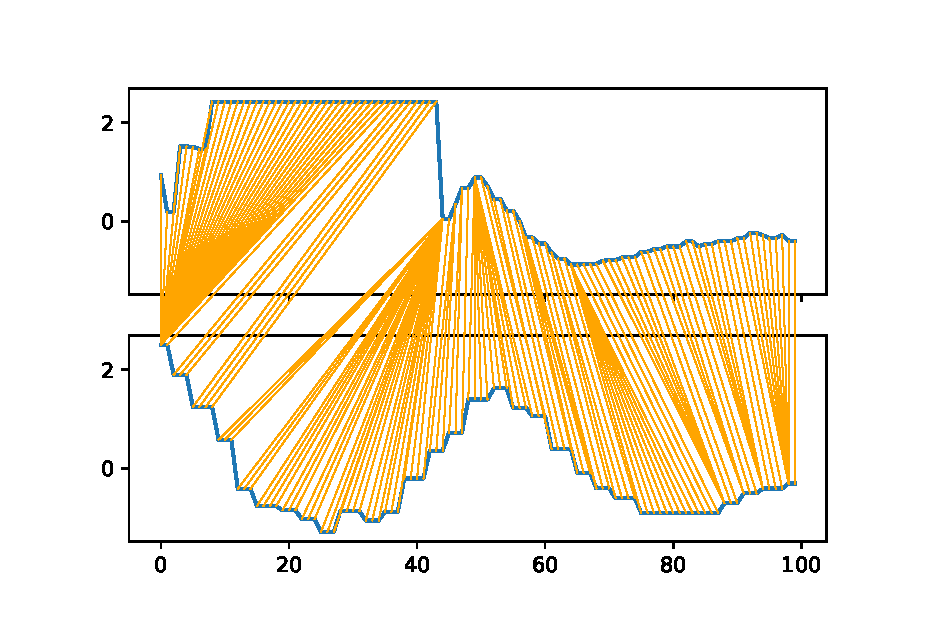
\includegraphics[width = \textwidth]{warp[1][3].eps}
\end{minipage}%
\caption{ . 2 и 4 временные ряды}
\label{fig:2}
\end{figure}

\begin{figure}[H]
\centering
\begin{minipage}{0.66\textwidth}
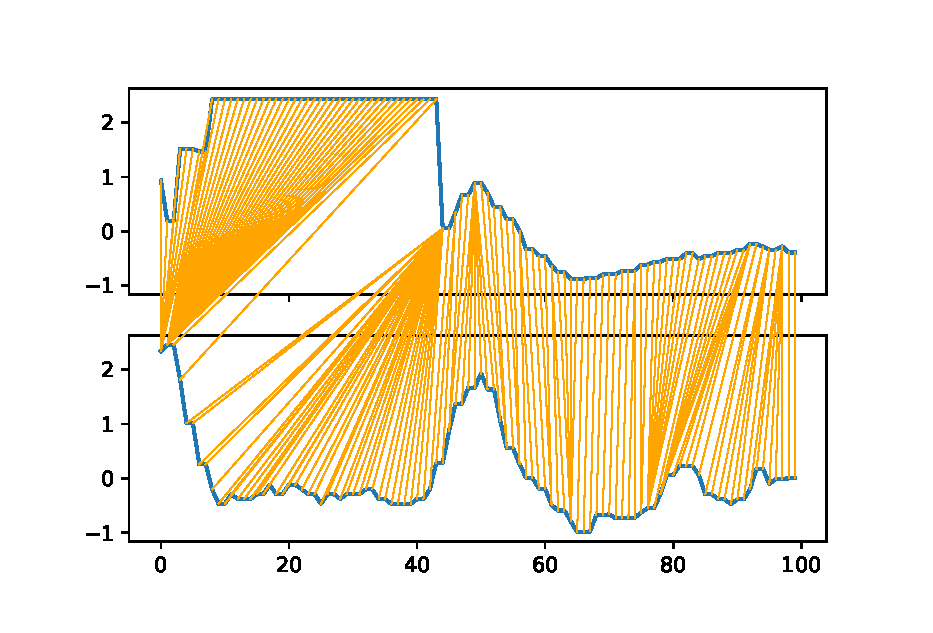
\includegraphics[width = \textwidth]{warp[1][4].eps}
\end{minipage}%
\caption{ . 2 и 5 временные ряды}
\label{fig:2}
\end{figure}

\begin{figure}[H]
\centering
\begin{minipage}{0.66\textwidth}
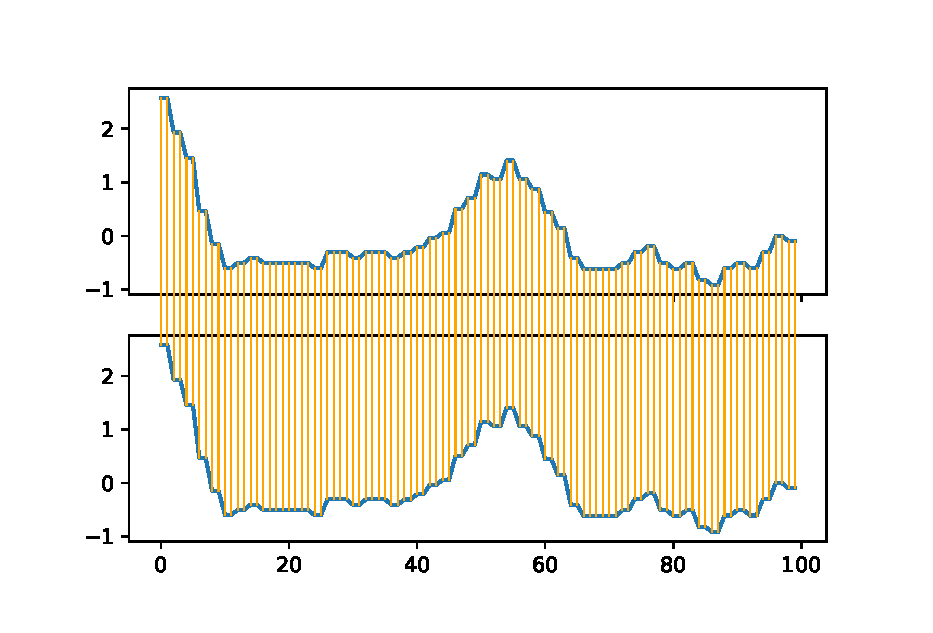
\includegraphics[width = \textwidth]{warp[2][2].eps}
\end{minipage}%
\caption{ . 3 и 3 временные ряды}
\label{fig:2}
\end{figure}

\begin{figure}[H]
\centering
\begin{minipage}{0.66\textwidth}
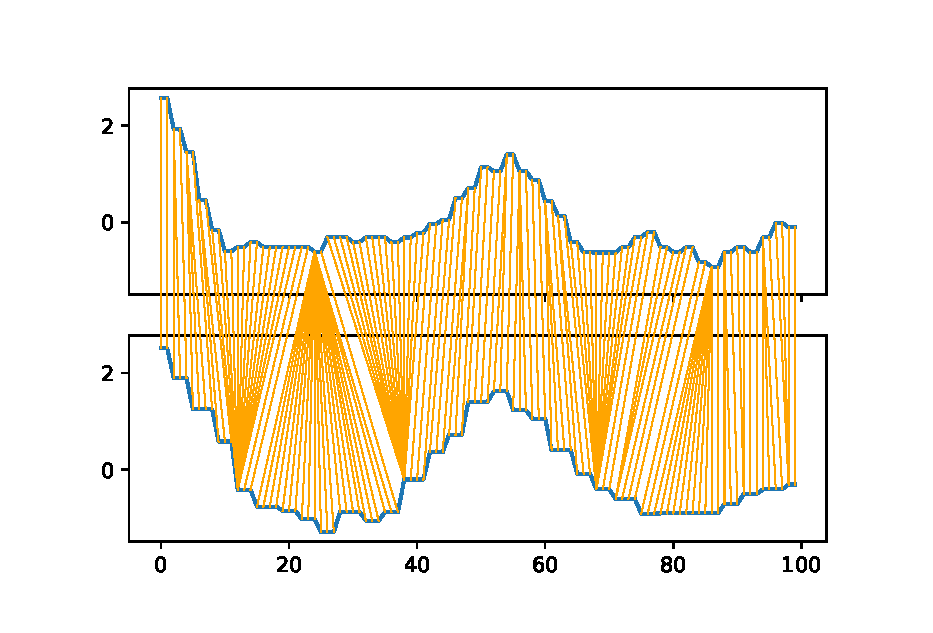
\includegraphics[width = \textwidth]{warp[2][3].eps}
\end{minipage}%
\caption{ . 3 и 4 временные ряды}
\label{fig:2}
\end{figure}

\begin{figure}[H]
\centering
\begin{minipage}{0.66\textwidth}
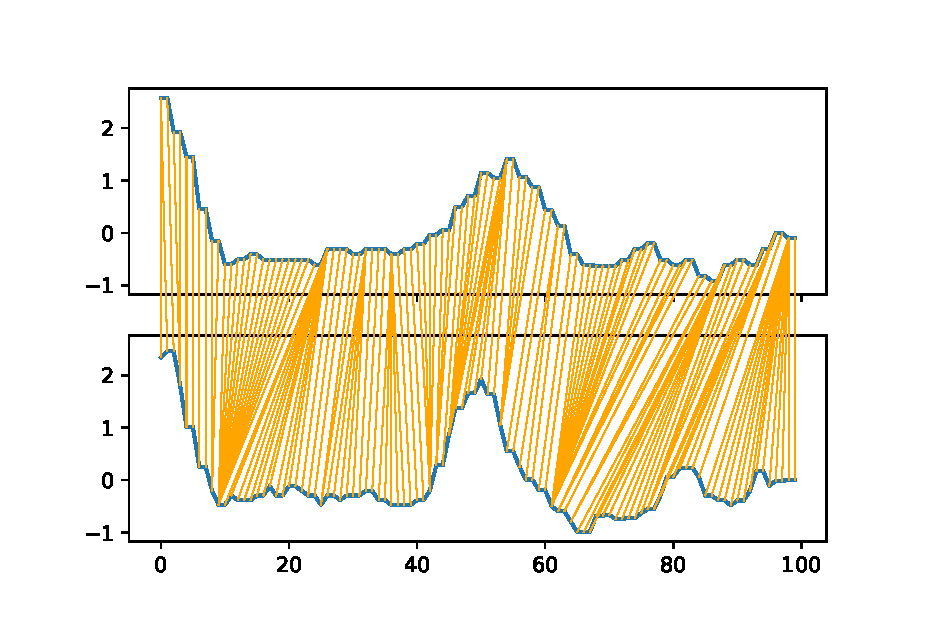
\includegraphics[width = \textwidth]{warp[2][4].eps}
\end{minipage}%
\caption{ . 3 и 5 временные ряды}
\label{fig:2}
\end{figure}

\begin{figure}[H]
\centering
\begin{minipage}{0.66\textwidth}
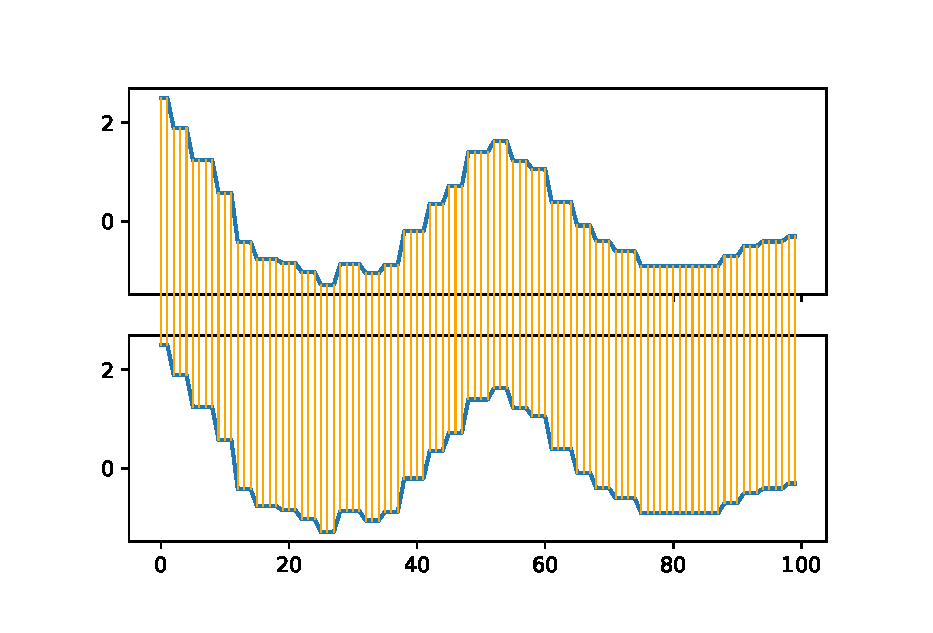
\includegraphics[width = \textwidth]{warp[3][3].eps}
\end{minipage}%
\caption{ . 4 и 4 временные ряды}
\label{fig:2}
\end{figure}

\begin{figure}[H]
\centering
\begin{minipage}{0.66\textwidth}
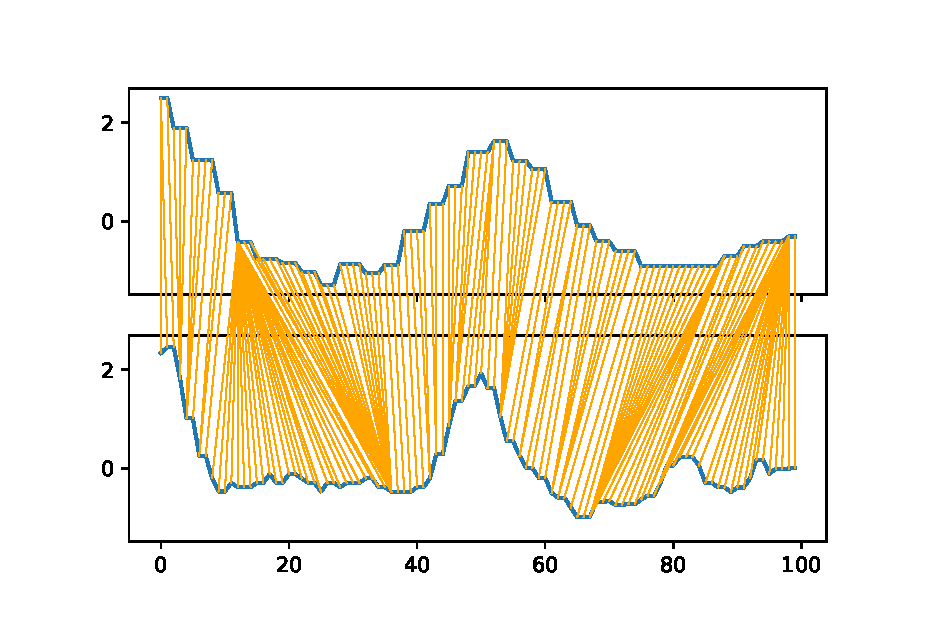
\includegraphics[width = \textwidth]{warp[3][4].eps}
\end{minipage}%
\caption{ . 4 и 5 временные ряды}
\label{fig:2}
\end{figure}


С помощью DTW посчитана матрица $D$ попарных расстояний между рядами.\\


\begin{figure}[H]
\centering
\begin{minipage}{0.76\textwidth}
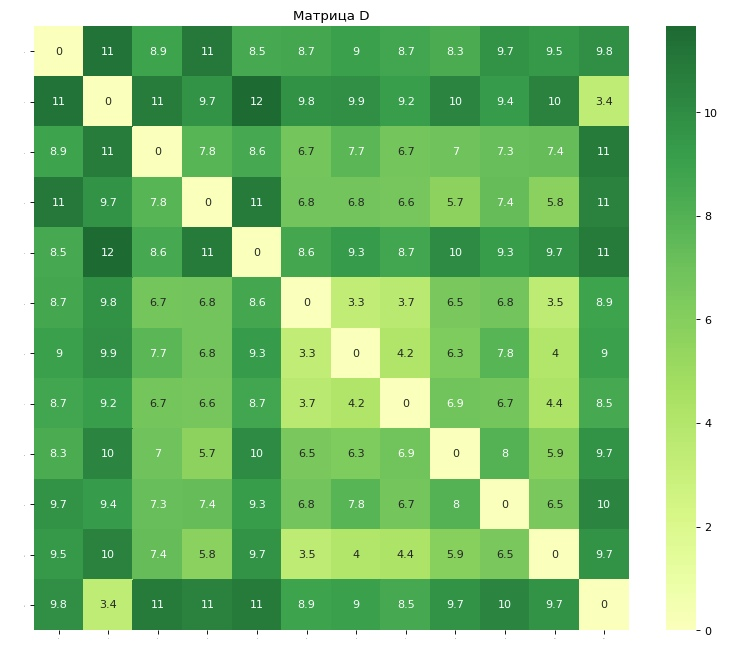
\includegraphics[width = \textwidth]{jmlda-guides/D.jpg}
\end{minipage}%
\caption{ .}
\label{fig:2}
\end{figure}




Матрица $D$ не является положительно полуопределенной ($\Rightarrow$ не является ядром), поэтому мы будем искать ближайшую к ней положительно полуопределенную матрицу $A$ следующим образом:
Так как матрица $D$ - симметричная, то разложим ее в таком виде $D = QMQ^T$, где матрица $M$ - диагональная, причем на диагонали стоят собственные значения матрицы $D$. Обозначим $M_{+} = max(M, 0)$, тогда $A = QM_{+}Q^T$. Матрица $A$ - положительно полуопределенная, так как все ее собственные значения - элементы диагональной матрицы $M_{+}$ неотрицательны.
\\

\begin{figure}[H]
\centering
\begin{minipage}{0.66\textwidth}
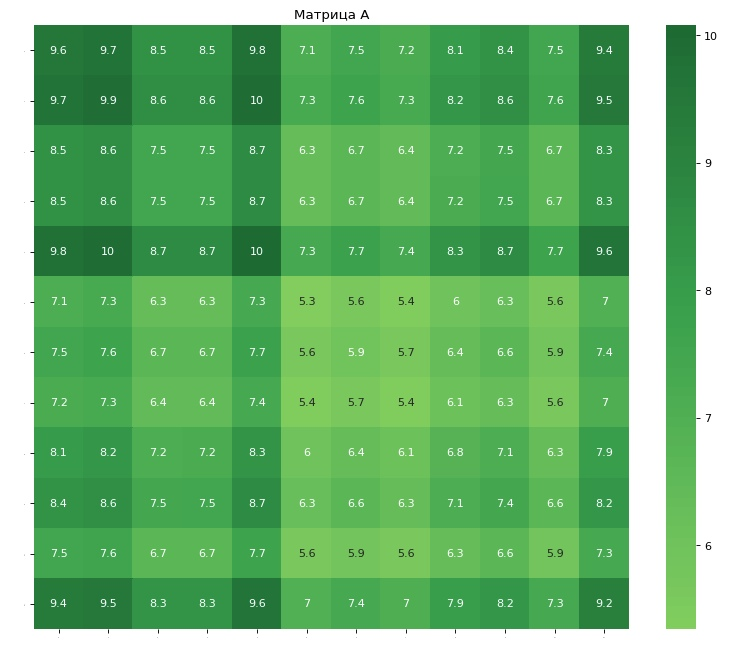
\includegraphics[width = \textwidth]{jmlda-guides/A.jpg}
\end{minipage}%
\caption{ . }
\label{fig:2}
\end{figure}

\\
{Эксперимент подтверждает, что матрица $A$ является положительно полуопределенной.}

{Также можно создавать RBF ядро $K(x, x') = exp(-\gamma \cdot \rho_{dtw}(x, x'))$, где $\rho_{dtw}(x, x')$ - расстояние между рядами $x$ и $x'$. Полученная матрица $Z$ также получится неотрицательно определенной.}\\

\begin{figure}[H]
\centering
\begin{minipage}{0.66\textwidth}
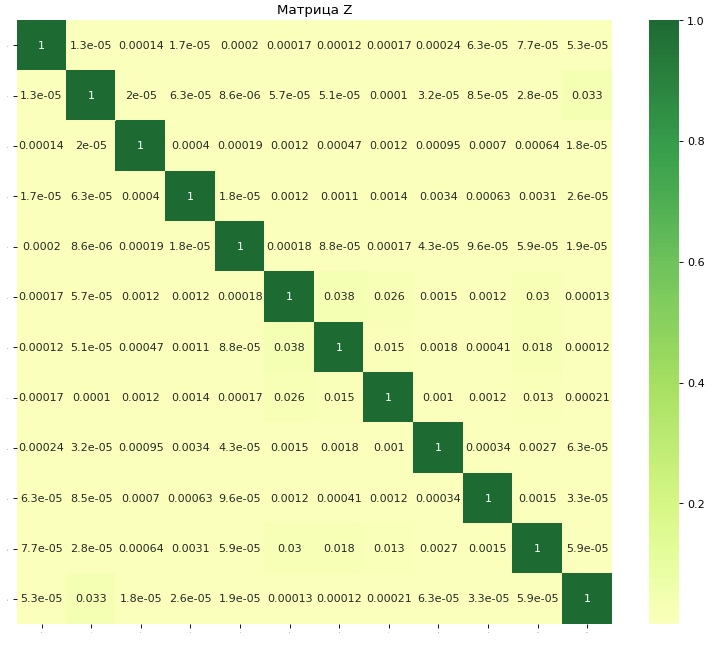
\includegraphics[width = \textwidth]{jmlda-guides/Z.jpg}
\end{minipage}%
\caption{ .}
\label{fig:2}
\end{figure}

{Затем, мы считаем таким же образом матрицы $D, \ A, \ Z$ для большего размера данных (временные ряды), а затем используем матрицы $D, \ A, \ Z$, а также просто норму $l_2$ в качестве "ядра"  в алгоритме SVM для их классификации.}\\
{И замеряем метрику качества, получаем следующие результаты:}\\
{$\bullet$ для $l_2: 0.182$}\\
{$\bullet$ для $D$ (просто DTW): $0.327$}\\
{$\bullet$ для $A$ (ближайшая к $D$ неотрицательно определенная): $0.523$}\\
{$\bullet$ для $Z$ (rbf ядро): $0.864$}\\



\section{Заключение}
Как и ожидалось, метрика $l_2$ дала худший результат, следующий результат дала матрица $D$, улучшив предыдущий на $20 \%$, затем матрица $A$ - аппроксимация $D$, улучшив результат еще на $20 \%$, и лучший результат дало RBF ядро $Z$.

%%%% если имеется doi цитируемого источника, необходимо его указать, см. пример в \bibitem{article}
%%%% DOI публикации, зарегистрированной в системе Crossref, можно получить по адресу http://www.crossref.org/guestquery/

%%%% если имеется doi цитируемого источника, необходимо его указать, см. пример в \bibitem{article}
%%%% DOI публикации, зарегистрированной в системе Crossref, можно получить по адресу http://www.crossref.org/guestquery/.

\bibliographystyle{plain}
\bibliography{litr}

\end{document}
